\documentclass[12pt,letterpaper]{article}
\usepackage[utf8]{inputenc}
\usepackage{amsmath,amssymb,fullpage,graphicx}
\usepackage{subfigure}
\usepackage{amssymb}
\let\hat\widehat
\let\tilde\widetilde


\author{Nan Tang\\1662478}
	%% your name
\title{STAT 403 Spring 2018\\HW02}
	%% title of this document
\begin{document}
\maketitle
	%% make the title and author

\section*{Q1}

\subsection*{Q1-1}

\begin{align*}
p(x) &= 
\begin{cases}
      6x(1-x), & \text{if}\ x \in [0, 1] \\
      1, & \text{otherwise}
\end{cases}
\end{align*}

\noindent For $x \in [1, 0]$, the cdf of X is 
\begin{align*}
F_X(x) &= \int_{0}^{x} p(t) dt\\
&= \int_{0}^{x} 6t(1-t) dt \\
&= \int_{0}^{x}6t - 6t^2 dt \\
&= 3x^2 - 2x^3
\end{align*}

\noindent Otherwise, if $x > 1, F(x) = 1$; if $x < 0, F(x) = 0$, since $p(x) = 0$ if $x \notin [0, 1]$.
\begin{align*}
F_X(x) &= 
\begin{cases}
      3x^2 - 2x^3, & \text{if}\ x \in [0, 1] \\
      1, & \text{if}\ x > 1 \\
      0, & \text{if}\ x < 0 
\end{cases}
\end{align*}

\subsection*{Q1-2}
\noindent For $x \in [0, 1]$, the edf of X is
\begin{align*}
\hat{F_n}(x) &= \frac{1}{n} \sum_{i=1}^{n} I(x_i \leq x)
\end{align*}

\begin{align*}
\mathbb{E}(\hat{F_n}) &= \mathbb{E}( \frac{1}{n} \sum_{i=1}^{n} I(x_i \leq x)) \\
&=  \frac{1}{n} \sum_{i=1}^{n} \mathbb{E}(x_i \leq x) \\
&=  \mathbb{E}(x_i \leq x) \\
&= P(x_i < x) \\
&= F_X(x) \text{, since $(x_i < x)$ follows Bernoulli distribution}\\
&= 3x^2 - 2x^3
\end{align*}

\begin{align*}
Var(\hat{F_n}) &= Var(\frac{1}{n} \sum_{i=1}^{n} I(x_i \leq x)) \\
&= \frac{1}{n^2} \sum_{i=1}^{n} Var(I(x_i \leq x)) \\
&= \frac{1}{n} Var(P(x_i < x)) \\
&= \frac{1}{n} F(x)(1 - F(x)) \text{, since } Var(Bern(p)) = p(1-p) \\
&= \frac{(3x^2 - 2x^3)(1 - 3x^2 + 2x^3)}{n}
\end{align*}

\pagebreak
\subsection*{Q1-3}
\begin{verbatim}
x_base <- seq(0, 1, 0.01)
beta_cdf <- function(x) {return(3 * x^2 - 2 * x^3)}
plot(x_base, beta_cdf(x_base), type='l', col='skyblue', lwd=3,
     xlim=c(0, 1), main='CDF of Beta(2, 2)', xlab='x value', ylab='F(x)')
\end{verbatim}

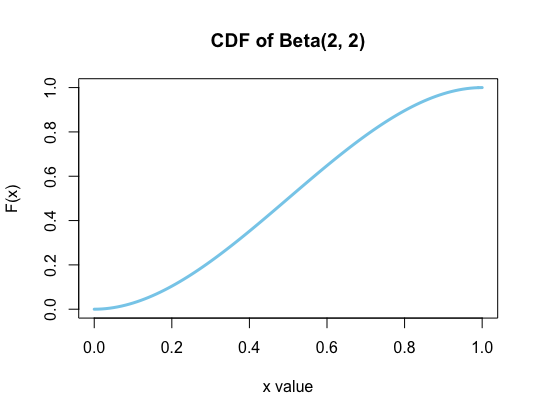
\includegraphics[width=150mm]{plot_beta.png}

\section*{Q2}
\subsection*{Q2-1}
Given $U \sim Uniform(0, 1) $ and $W = -2log(U)$. \\
\noindent The cdf of U $F_U(x) = x, x \in [0, 1]$. \\
\noindent First find the cdf of W.
\begin{align*}
F_W(x) &= P(W < x) \\
P(W < x) &= P(-2log(U) < x) \\
&= P(e^{-2log(U)} < e^x) \\
&= P(U^{-2} < e^x) \\
&= P(U \geq e^{- \frac{x}{2}}) \\
&= 1 - P(U < e^{- \frac{x}{2}}) \\
&= 1 - e^{- \frac{x}{2}}
\end{align*}

\noindent Note that the cdf of $Exp(0.5)$, $F = 1 - e^{- \frac{x}{2}}$, which is equal to the cdf of $W$, therefore, we can conclude that $W$ and $Exp(0.5)$ have the same distribution. 

\





%%% do not touch anything below
\end{document}
